\documentclass[border=10pt]{standalone}
\usepackage{pgfplots}
\pgfplotsset{compat=1.18}

\begin{document}
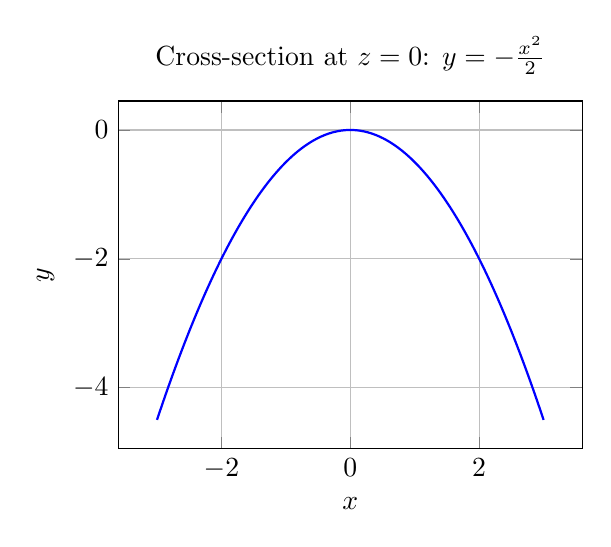
\begin{tikzpicture}
\begin{axis}[
    xlabel={$x$},
    ylabel={$y$},
    title={Cross-section at $z = 0$: $y = -\frac{x^2}{2}$},
    domain=-3:3,
    samples=100,
    width=8cm,
    height=6cm,
    grid=major,
    axis equal image,
]
\addplot[blue, thick, smooth] {-x^2/2};
\end{axis}
\end{tikzpicture}
\end{document}